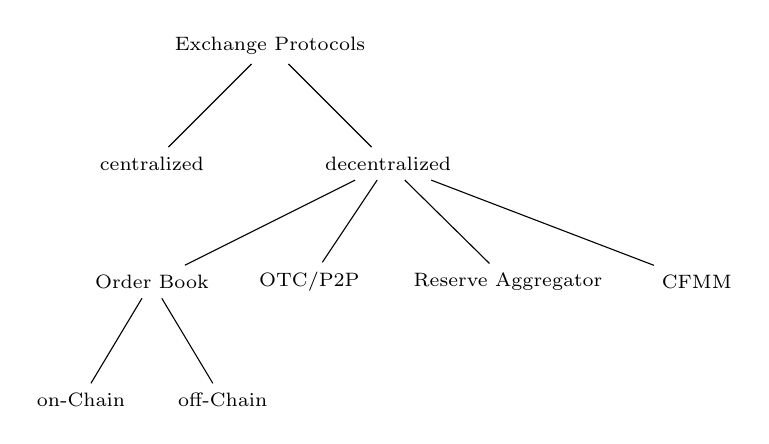
\begin{tikzpicture}
		[ sibling distance =10em ,
		every node/.style = {%shape=rectangle, rounded corners,
		%draw,
		font=\scriptsize,
		align = center,
		%top color=white, bottom color = highlight
		}]]
 		\tikzstyle{level 1}=[sibling distance=30mm]
 		\tikzstyle{level 2}=[sibling distance=20mm]
 		\tikzstyle{level 3}=[sibling distance=18mm]
  
  			\node {Exchange Protocols}
  			child { node {centralized}}
  			child { node {decentralized}
  				child { node {Order Book}
  					child { node {on-Chain}}
  					child { node {off-Chain}}}
  				child { node {OTC/P2P}}
  				child { node[right=-8mm] {Reserve Aggregator}}
  				child { node[right=1em] {CFMM}}
  			};
		\end{tikzpicture}